\author{Gottfried von Recum}

\section{Browser}

Denkbare Use Cases des Browsers sind:
\begin{figure}[h]
	\centering
	\includegraphics[width=0.6\textwidth]{use_case_browser1}
	\caption{Menüführung des Browsers (Navigation)}
	\label{fig:Browser Navigation}
\end{figure}

Dieses Use-Case Diagramm zeigt die wesentlichen Funktionen des Browsers auf einer Homepage eine Seite zurück zu gehen oder eine Seite vor zu wechseln. Im weiteren hat er die Möglichkeit ein eigenes Lesezeichen anzulegen.

\begin{figure}[h]
	\centering
	\includegraphics[width=0.6\textwidth]{use_case_browser2}
	\caption{Lesezeichenverwaltung des Browsers}
	\label{fig:Browser Lesezeichen}
\end{figure}

In diesem Use-Case Diagramm wird die Lesezeichenverwaltung veranschaulicht. Der Nutzer kann ein angelegtes Lesezeichen auswählen, diese löschen oder editieren.

\begin{figure}[h]
	\centering
	\includegraphics[width=0.6\textwidth]{use_case_browser3}
	\caption{URL Navigation und \SECH-Tabelle des Browsers}
	\label{fig:Browser URL}
\end{figure}

Dieses Use-Case Diagramm zeigt weitere Navigationselemente im Browser. Er kann die von ihm definierte Startseite laden, eine URL in die Suchleiste eingeben und bestätigen oder die aktuelle Seite neu laden und die Optionen öffnen. Des Weiteren kann er die \SECH-Tabelle ein- und ausfahren in der sich die \SECH-Tags befinden und er eines dieser auswählen kann.

\begin{figure}[h]
	\centering
	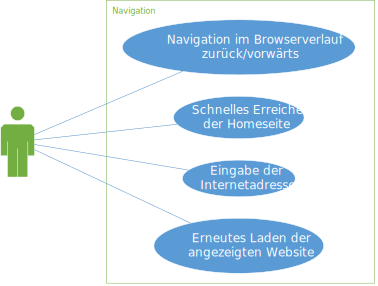
\includegraphics[width=0.6\textwidth]{USECASE_Nutzer_Browser_Navigation}
	\caption{Use Case der Browser Navigation}
	\label{fig:Browser Navigation Use-Case}
\end{figure}

\begin{figure}[h]
	\centering
	\includegraphics[width=0.6\textwidth]{USECASE_Nutzer_Lesezeichen}
	\caption{Use Case der Browser Lesezeichen}
	\label{fig:Browser Lesezeichen Use-Case}
\end{figure}

\begin{figure}[h]
	\centering
	
\includegraphics[width=0.6\textwidth]{USECASE_Nutzer_Einstellungen}
	\caption{Use Case der Browser Einstellungen}
	\label{fig:Browser Einstellungen Use-Case}
\end{figure}